% Status info:
% M. Gates	2006-2009
% A. Wolf	2011-2015
% ArdWar	2012
% B. Gerdes	2013
% TODO insert further additions from wiki?
% GZ Content OK for 0.15+.
% 20160329 GZ: typo&grammar check 
% 20160407 GZ: Split Bortle Scale into chapter for reference appendix
% 20170416 AW: Updated data from Wikipedia, added references, added image

\chapter{The Bortle Scale of Light Pollution}
\label{ch:BortleScale}

The Bortle scale is a nine-level numeric scale that 
measures the night sky's brightness of a particular 
location. It quantifies the astronomical observability 
of celestial objects and the interference caused by 
light pollution. \name{John E.\ Bortle} created the 
scale and published it in \emph{Sky \& Telescope} 
magazine to help amateur astronomers evaluate the 
darkness of an observing site, and secondarily, 
to compare the darkness of observing sites. The 
scale ranges from Class 1, the darkest skies available 
on Earth, through Class 9, inner-city skies. 
It gives several criteria for each level beyond 
naked-eye limiting magnitude (NELM)~\cite{Bortle}. 
The accuracy and utility of the scale have been questioned in 
recent research~\cite{2014MNRAS.442.2600C}.

\begin{figure}[ht]\centering
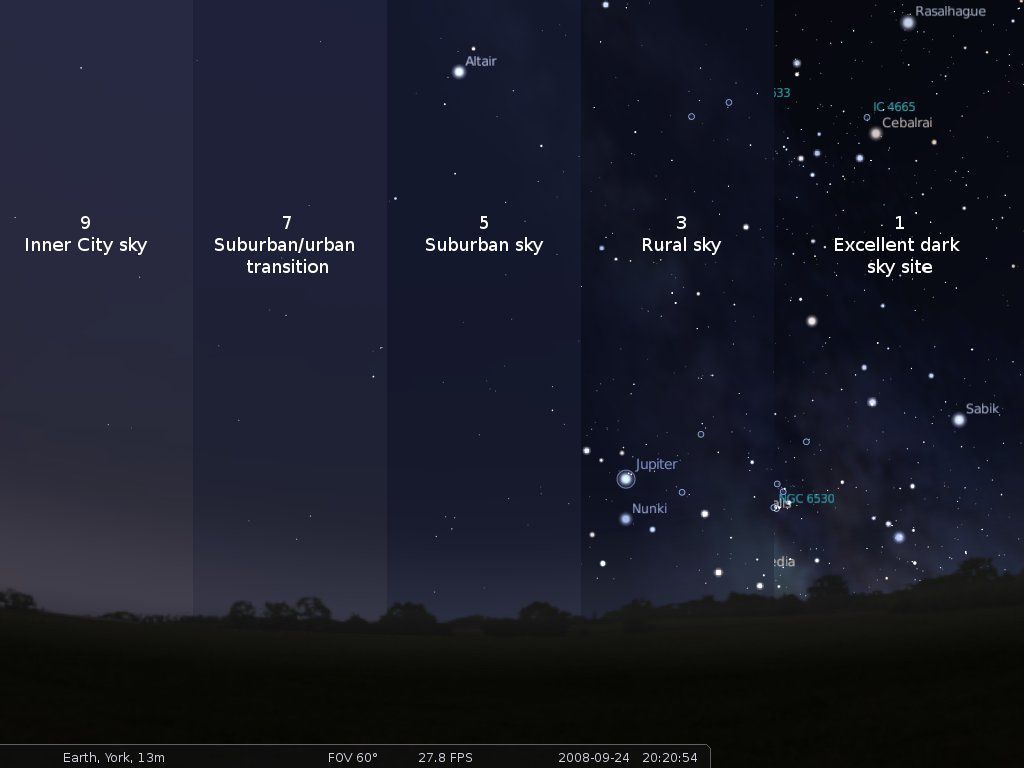
\includegraphics[trim=0 55 0 0,clip,width=\textwidth]{bortle_scale.jpg}
\caption{Light Pollution Simulation / Bortle Scale}
\label{fig:BortleScale}
\end{figure}

\section{Excellent dark sky site}
\textbf{Level:} 1 \\
\textbf{Naked-eye limiting magnitude:} 7.6 -- 8.0 \\
\textbf{Approx. SQM mag/arcsec$^2$:} 21.7 -- 22.0\footnote{Dark Skies Awareness -- \url{http://www.darkskiesawareness.org/nomogram.php}}

Zodiacal light, gegenschein, zodiacal band visible; M33 direct vision
naked-eye object; Scorpius and Sagittarius regions of the Milky Way
cast obvious shadows on the ground; Airglow is readily visible;
Jupiter and Venus affect dark adaptation; surroundings basically
invisible.

\section{Typical truly dark site}
\textbf{Level:} 2 \\
\textbf{Naked-eye limiting magnitude:} 7.1 -- 7.5 \\
\textbf{Approx. SQM mag/arcsec$^2$:} 21.5 -- 21.7

Airglow weakly visible near horizon; M33 easily seen with naked eye;
highly structured Summer Milky Way; distinctly yellowish zodiacal
light bright enough to cast shadows at dusk and dawn; clouds only
visible as dark holes; surroundings still only barely visible
silhouetted against the sky; many Messier globular clusters still
distinct naked-eye objects.

\section{Rural sky}
\textbf{Level:} 3 \\
\textbf{Naked-eye limiting magnitude:} 6.6 -- 7.0 \\
\textbf{Approx. SQM mag/arcsec$^2$:} 21.3 -- 21.5

Some light pollution evident at the horizon; clouds illuminated near
horizon, dark overhead; Milky Way still appears complex; M15, M4, M5,
M22 distinct naked-eye objects; M33 easily visible with averted
vision; zodiacal light striking in spring and autumn, color still
visible; nearer surroundings vaguely visible.

\section{Rural/suburban transition}
\textbf{Level:} 4 \\
\textbf{Naked-eye limiting magnitude:} 6.1 -- 6.5 \\
\textbf{Approx. SQM mag/arcsec$^2$:} 20.4 -- 21.3

Light pollution domes visible in various directions over the horizon;
zodiacal light is still visible, but not even halfway extending to the
zenith at dusk or dawn; Milky Way above the horizon still impressive,
but lacks most of the finer details; M33 a difficult averted vision
object, only visible when higher than 55$\degree$; clouds illuminated
in the directions of the light sources, but still dark overhead;
surroundings clearly visible, even at a distance.

\newpage
\section{Suburban sky}
\textbf{Level:} 5 \\
\textbf{Naked-eye limiting magnitude:} 5.6 -- 6.0 \\
\textbf{Approx. SQM mag/arcsec$^2$:} 19.1 -- 20.4

Only hints of zodiacal light are seen on the best nights in autumn and
spring; Milky Way is very weak or invisible near the horizon and looks
washed out overhead; light sources visible in most, if not all,
directions; clouds are noticeably brighter than the sky.

\section{Bright suburban sky}
\textbf{Level:} 6 \\
\textbf{Naked-eye limiting magnitude:} 5.1 -- 5.5 \\
\textbf{Approx. SQM mag/arcsec$^2$:} 18.0 -- 19.1

Zodiacal light is invisible; Milky Way only visible near the zenith;
sky within 35$\degree$ from the horizon glows grayish white; clouds
anywhere in the sky appear fairly bright; surroundings easily visible;
M33 is impossible to see without at least binoculars, M31 is modestly
apparent to the unaided eye.

\section{Suburban/urban transition}
\textbf{Level:} 7 \\
\textbf{Naked-eye limiting magnitude:} 4.6 -- 5.0 \\
\textbf{Approx. SQM mag/arcsec$^2$:} 18.0 -- 19.1

Entire sky has a grayish-white hue; strong light sources evident in
all directions; Milky Way invisible; M31 and M44 may be glimpsed with
the naked eye, but are very indistinct; clouds are brightly lit; even
in moderate-sized telescopes the brightest Messier objects are only
ghosts of their true selves.

\section{City sky}
\textbf{Level:} 8 \\
\textbf{Naked-eye limiting magnitude:} 4.1 -- 4.5 \\
\textbf{Approx. SQM mag/arcsec$^2$:} <18.0

Sky glows white or orange --- you can easily read; M31 and M44 are
barely glimpsed by an experienced observer on good nights; even with
telescope, only bright Messier objects can be detected; stars forming
familiar constellation patterns may be weak or completely invisible.

\section{Inner-city sky}
\textbf{Level:} 9 \\
\textbf{Naked-eye limiting magnitude:} 4.0 at best \\
\textbf{Approx. SQM mag/arcsec$^2$:} <18.0

Sky is brilliantly lit with many stars forming constellations
invisible and many weaker constellations invisible; aside from
Pleiades, no Messier object is visible to the naked eye; only objects
to provide fairly pleasant views are the Moon, the Planets and a few
of the brightest star clusters.


%%% Local Variables: 
%%% mode: latex
%%% TeX-master: "guide"
%%% End: 

